\section{Overview}

The system's development and testing will follow a feature-based, bottom-up approach combined with threading. This hybrid strategy ensures systematic integration while making visible progress, leveraging the strengths of both methodologies.

Within each feature thread, the bottom-up strategy is applied by developing and testing the lowest-level components first (e.g., CoreEntityManager in Feature 1) using drivers to simulate higher-level components. Incrementally, higher-level components like MainPlatform are developed and tested with drivers for components such as FrontendInterface. This approach eliminates the need for stubs and facilitates early verification of critical modules, ensuring a stable foundation for higher-level functionality.

Threading complements this by integrating modules that deliver user-visible functionality. It accelerates progress visibility, aligns each thread with specific features (e.g., Internship Matching), and reflects real-world workflows, especially for complex module interactions like NotificationHandler, InterviewHandler, and FrontendInterface.

Together, these strategies create robust building blocks, accelerate feature delivery, and maintain stakeholder confidence. This hybrid approach supports rigorous verification of components and rapid development of user-facing features, aligning with the system’s architecture and requirements \cite{Camilli2024}.

\section{Implementation Plan}

This section specifies the implementation plan.

First, the main features (identified in the Functional Requirements section of the RASD \cite{ContiMarino2024}) are sorted according to the number of components involved (see \hyperref[ch:requirements_traceability]{Requirements Traceability}). However, we do not assume sequential development—features can be developed in parallel by multiple teams to accelerate progress.

\subsubsection{Feature Identification and Sorting}
\begin{enumerate}[label={[F\arabic*]}]
    \item \textbf{Internship Publication and Management} \\ This feature enables companies to publish, manage, and cancel internship opportunities. It includes input verification, ensuring correctness and completeness of internship data. It is prioritized as it involves fewer components, is critical for building the internship database, and is relatively straightforward compared to subsequent features.
    \item \textbf{Search and Apply for Internships} \\ This feature allows students to search and apply for internships using filters like role and location. It includes mechanisms to ensure accurate search results and simple application processes. This comes next as it adds functionality to the published internships, has a moderate number of components, and is critical for student interaction.
    \item \textbf{Internship Matching and Recommendation} \\  This feature leverages external systems to recommend internships to students and suggest suitable candidates to companies. It relies on existing internship and student profiles. It follows as it is more complex, uses more components, and builds upon the foundational features of publication and searching. Also, we hope it acts as a wow-factor for stakeholders.
    \item \textbf{Sign-Up, Login and Profile Management}\\ This feature handles user authentication and profile creation for both students and companies. Profiles include critical data like skills, preferences, and organizational details. This is introduced later as it is less critical initially and involves multiple components.
    \item \textbf{Interview Management and Selection Process} \\ This feature allows scheduling, conducting, and managing interviews. It incorporates availability management and communication via notifications. It is placed here as it is more complex, uses many components, and relies on established profiles, internships, and matchmaking capabilities.
    \item \textbf{Feedback and Complaint Management} \\ This feature facilitates post-internship feedback and complaint filing for ongoing internships. It is implemented last as it is the least critical initially, highly dependent on previous functionalities, and involves a greater number of interactions and components.
\end{enumerate}


\section{Component Integration and Testing}

\subsubsection{[F1] Internship Publication and Management}

\begin{figure}[H]
    \centering
    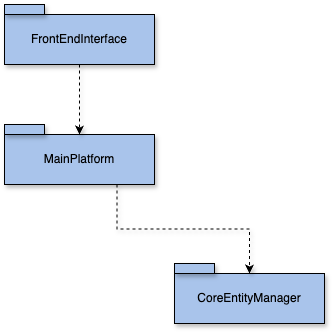
\includegraphics[width=0.5\textwidth]{Images/implementation-testing-hierarchy_f1.png}
    \caption{Components developed in Feature 1}
    \label{fig:implementation_testing_f1}
\end{figure}

The highlighted components in this diagram focus on enabling companies to publish, manage, and cancel internship opportunities. Integration testing involves validating the seamless communication between the FrontEndInterface, MainPlatform, and CoreEntityManager. Tests ensure that input validation, data persistence, and feedback to users function as intended. Mock data is used to simulate internship submissions, and edge cases like missing fields or incorrect formats are checked to confirm the robustness of the feature.

\subsubsection{[F2] Search and Apply for Internships}

\begin{figure}[H]
    \centering
    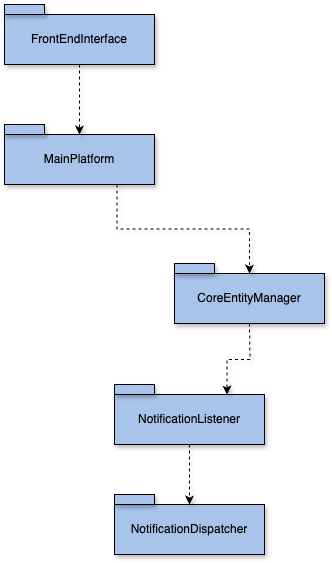
\includegraphics[width=0.5\textwidth]{Images/implementation-testing-hierarchy_f2.png}
    \caption{Components developed in Feature 2}
    \label{fig:implementation_testing_f2}
\end{figure}

The diagram highlights components responsible for retrieving and displaying internships based on user criteria. Testing includes verifying the CoreEntityManager's ability to process search filters and return results efficiently. The interaction between the MainPlatform and the FrontendInterface is tested to confirm accurate display of data. Applying for an internship is tested by ensuring the CoreEntityManager logs applications correctly and triggers appropriate user notifications.


\subsubsection{[F3] Internship Matching and Recommendation}

\begin{figure}[H]
    \centering
    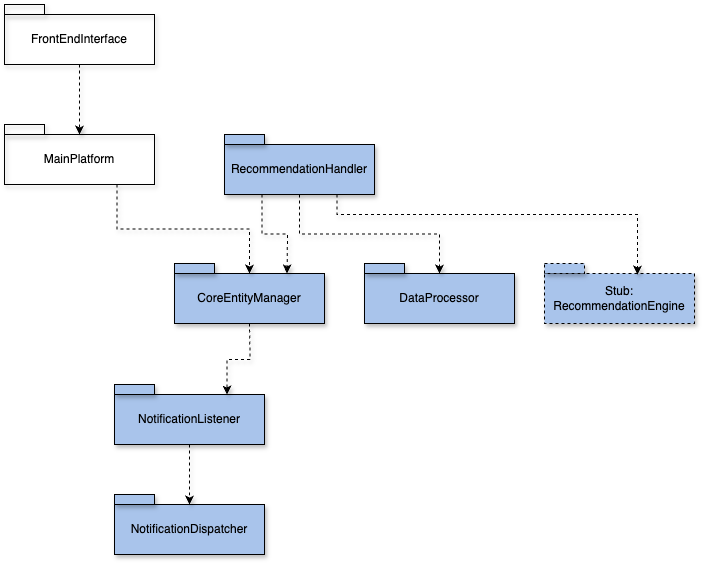
\includegraphics[width=\textwidth]{Images/implementation-testing-hierarchy_f3.png}
    \caption{Components developed in Feature 3}
    \label{fig:implementation_testing_f3}
\end{figure}

This diagram showcases the components involved in recommending internships to students and suggesting candidates to companies. Testing focuses on the integration between the RecommendationScheduler, CoreEntityManager, DataProcessor, and the RecommendationEngine. Tests validate that preprocessing steps filter data accurately and that the external recommendation engine returns valid matches. Notification dispatch for recommendations is tested for timely and correct delivery.

\subsubsection{[F4] Sign-Up, Login and Profile Management}

\begin{figure}[H]
    \centering
    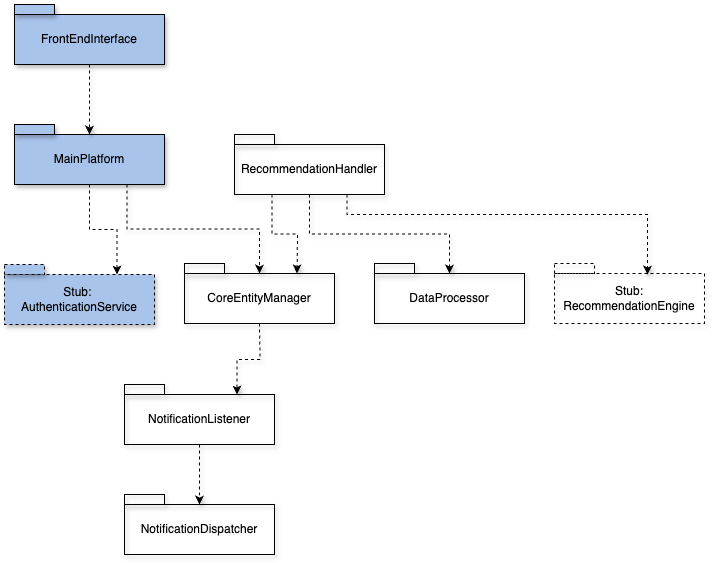
\includegraphics[width=\textwidth]{Images/implementation-testing-hierarchy_f4.png}
    \caption{Components developed in Feature 4}
    \label{fig:implementation_testing_f4}
\end{figure}

The components in this feature enable user registration, authentication, and profile management. Integration tests validate the AuthenticationService for secure handling of user credentials and the CoreEntityManager for storing profile data. Scenarios such as duplicate accounts, incorrect credentials, and partial profile submissions are used to confirm system reliability.

\subsubsection{[F5] Interview Management and Selection Process}

\begin{figure}[H]
    \centering
    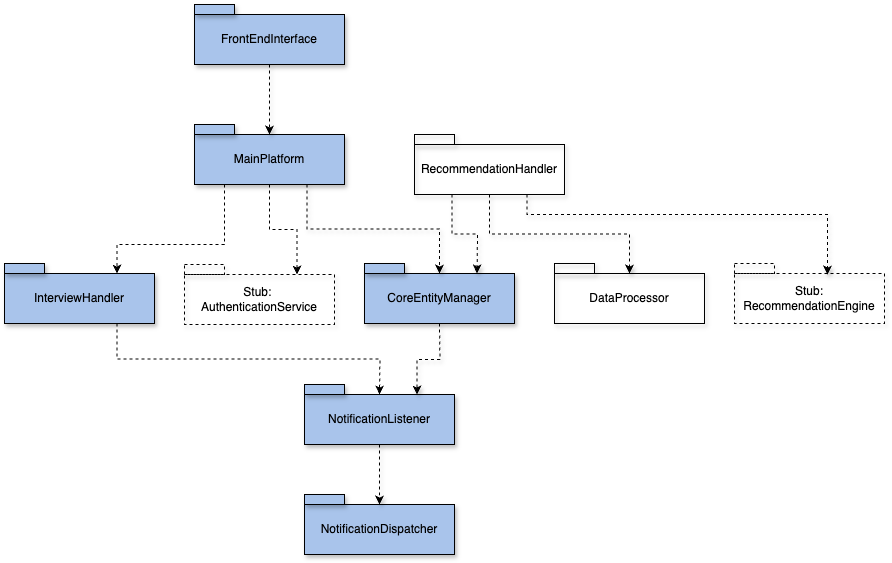
\includegraphics[width=\textwidth]{Images/implementation-testing-hierarchy_f5.png}
    \caption{Components developed in Feature 5}
    \label{fig:implementation_testing_f5}
\end{figure}

The highlighted components manage scheduling, conducting, and updating interviews. Testing ensures proper communication between the FrontendInterface, MainPlatform, and InterviewHandler. Scenarios include creating, confirming, and canceling interviews, with checks for correct notification triggers. The InterviewHandler is also tested for accurately maintaining availability slots and recording outcomes.

\subsubsection{[F6] Feedback and Complaint Management}

\begin{figure}[H]
    \centering
    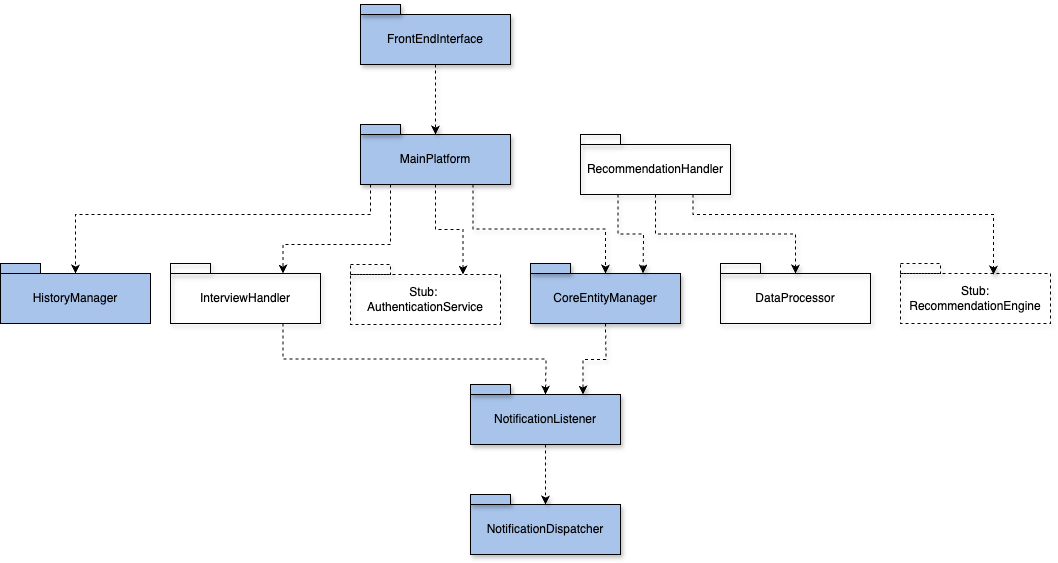
\includegraphics[width=\textwidth]{Images/implementation-testing-hierarchy_f6.png}
    \caption{Components developed in Feature 6}
    \label{fig:implementation_testing_f6}
\end{figure}

This feature integrates components to handle user feedback and complaints. Testing involves ensuring the HistoryManager accurately stores feedback and complaints and that the NotificationListener triggers appropriate alerts. The flow from form submission via the FrontendInterface to data persistence in the CoreEntityManager is validated for reliability and responsiveness.

\section{System Testing}
It is also of uttermost importance that the system is tested is as a whole and not only as separate components, since this complete use  is itself the ultimate goal of a project and the product visible to the user. As mentioned earlier, during the component testing some missing (i.e not yet developed) components may be replaced by stubs and drivers to test the target component. However, even after this test the component must be ensured to work well when integrated with the whole system, which is the purpose of the testing described here.

This means that, once a component is carefully tested as stated before, it can be integrated to the whole platform. Before this new version of the platform is considered an official release, it must undergo additional testing that ensures the fullfilment of the requirements provided on the RASD and not to jeopardize the fullfilment of requirements and behaviour of previous versions or instances of the program.
\subsection{Function Requirements Verification}
Functional Requirements Verification is the first necessary system testing and can be done simply using the software on each use-case and check whether or not it fullfills the specified requirements. The test cases may also be automated so to generate larger and less trivial scenarios corresponding to the specified use cases.
\subsection{Performance Testing}
Performance Testing is useful not only to detect the failure to meet non-functional requirements, but also detect excessively inefficient algorithms and procedures that may lead to bottlenecks on response time, utilization, and throughput. It is also important since, even if a non functional requirement is met on all tested scenarios, the replication and load balancing scheme could lead to a naive use of an inefficient algorithm and, even if it doesnt crash the program, may increase its operation cost. In this phase of testing the workload used is close to expected, and the performance is carefully taken account of to measure a typical usage case.
\subsection{Load Testing}
Load Testing conssits in rising the load from the previous typical usage to identify upper limits of components and subsystems and may lead to architectural changes. The system can be tested with an increased workload until it cannot support or its perfomance metrics become unacceptable. Not only the tested load is increased, but also the testing period, to see how it reacts to increased workloads in larger periods of time, if it balances itself well, if any useless resources remain in use etc. Since this is the sort of testing that can expose memory leaks and buffer overflows, it can also include a layer of fuzziness, in which random inputs are created to see how the system reacts. This is specially useful forthe global interaction of components such as the MainPlatform that have direct access to the FrontEndInterface, but also CoreEntityManager and InterviewHandler that have API calls from the FrontEndInterface through  the MainPlatform (that may not parse the calls appropriately before passing forward, depending on its development - and this would not necessarily be showed by the component testing). Also, the fuzzer can implement a mutation fuzzing from the automated test cases, so to predict common mistakes of the user such as typos or misclicks in certain moments.
\subsection{Stress Testing}
Stress Testing is useful to foresee how the system would react to extreme usage of resources and/or resource crashes - it comprises the matter of failure resistance. In this case, the interfaces can be stressed overwhelming the HTTPS/REST API calls, the replicated components can be diminished and even brought down to zero. Also, the network components can also be subject of stress testing, such as by limiting speeds, and randomly restarting routers. The replicated resources, even if they use open-source frameworks that guarantee some homogeneity, consistency and good replication schemes, can be tested by bringing down essential components randomly, such as the load balancer.
\section{Additional Specification on Testing}
Not only should the system be verified for internal coherence, but it should also be validated for external coherence, that is, to check whether or not it corresponds to the view and demand of users and other stakeholders. To do that, new developed features can go through alpha and beta testing. Once the system verification is done, that version becomes an update - but before being an official release it goes thorugh alpha and beta testing. Alpha testing includes the typical usage with that version of the product by the people directly related to its development, while beta testing opens up to people unrelated to the developed before an official release. 

While this is done to every crucial feature, the specifics and tweaks of every other added eature, for example the email format or the UI page for the recommendation feature, can be added first to target groups to test their experience and feedbacks before becoming a global feature. This takes addvantage of the thread-driven verification to validate parts of whole functionalities and experiences also separately from the whole user group, so to develop a better user experience and understand the users and stakeholders needs while deploying the product.